\chapter{Analytical Solutions for Structure factors}
\label{sec:structurefactor}
The different types of structure factors can be selected in the
different submenus. Next top traditional structure factors also
some functions, which are not structure factors
at all have been implemented for some other purposes.

\section{Methods to include structure factors}
For each scattering object $i$ next to a size distribution $N_i(x;\B{l}_i)$ also a
structure factor $S_i(Q;\B{s}_i)$ can be included. When a structure factor is included
several theoretical ways to account for it have been implemented
like the monodisperse approximation (\ref{sec:SQmonodisperse}),
decoupling approach (\ref{sec:SQdecoupling}),
local monodisperse approximation (\ref{sec:SQlocalmonodisperse}),
partial structure factor (\ref{sec:SQpartial})
and scaling approximation of partial structure factors (\ref{sec:SQscaling}).
At the moment it is assumed that there are no interactions between different species
of scatterers so that the total scattering is given by the sum of the scattering of the
individual species
\BE
\frac{d\sigma}{d\Omega}(Q) = \sum\limits_{i=1}^N \frac{d\sigma_i}{d\Omega}(Q)
\EE
whereby different approaches to include structure factor effects in
the differential scattering cross-sections $\frac{d\sigma_i}{d\Omega}(Q)$
of the species $i$ of scatterer are defined below.

\subsection{Monodisperse approach}
\label{sec:SQmonodisperse}
~\\

The monodisperse approach is the simplest way to include a structure factor in the analysis.
This approach simply multiplies the size averaged form factor with the structure factor.
Here it is assumed that the interaction potential between particles are spherical symmetric
and independent of the particle size.

\BE \frac{d\sigma_i}{d\Omega}(Q) = \left[
\int_0^\infty N_i(x;\B{l}_i)
F_i^2(Q;\B{a}_i,x) dx \right] S_i(Q;\B{s}_i)
\EE

\subsection{Decoupling approximation}
\label{sec:SQdecoupling}
~\\

For systems with small polydispersities and small anisotropies leads to a
decoupling approach of Kotlarchyk and Chen \cite{Kotlarchyk1983}. It is assumed that interactions
are independent of particle size and orientation.
%\begin{subequations}
\begin{align}
\frac{d\sigma_i}{d\Omega}(Q) = &
\int_0^\infty N_i(x;\B{l}_i) F_i^2(Q;\B{a}_i,x) dx
+  \frac{1}{n_i}\left[\int_0^\infty N_i(x;\B{l}_i)
F_i(Q;\B{a}_i,x) dx\right]^2  \nonumber \\
\times & \left[S_i(Q;\B{s}_i)-1\right]
\end{align}
with
\BE
n_i = \int_0^\infty N_i(x;\B{l}_i)  dx.
\label{eq:ni}
\EE

The decoupling approximation can only be combined with those form factor,
for which the scattering amplitude $F_i(Q;\B{a}_i,x)$ has been implemented.
However, for many form factors only the scattering intensity $F_i^2(Q;\B{a}_i,x)$ is
available. The combination of those form factors with the decoupling approach produces
an error message in \SASfit.



\subsection{Local monodisperse approximation}
\label{sec:SQlocalmonodisperse}
~\\

The opposite limit of the approximations as used for the
decoupling approximation is used in the local monodisperse
approximation \cite{Pedersen1994}. In this approach it is assumed
that a particle of a certain size is always surrounded by
particles with the same size. Following this the scattering is
approximated by that of monodisperse sub-systems weighted by the
size distribution:
\BE
\frac{d\sigma_i}{d\Omega}(Q) =
\int_0^\infty N_i(x;\B{l}_i)
F_i^2(Q;\B{a}_i,x) S_i(Q;\B{s}_i,R_i(\B{a}_i,x)) dx
\EE
in which it has been indicated that the structure factor is for particles of size
$R_i(\B{a}_i,x)$. As the distribution $N_i(x;\B{l}_i)$ does not necessarily describe the
distribution of the overall size. \SASfit assumes, that the radius of a particle
with the form factor $F_i(Q;\B{a}_i,x)$ used in the structure factor is given
by the radius of a sphere with the same volume $V_i(\B{a}_i,x)$
\BE
R_i(\B{a}_i,x) = \oldsqrt[3]{\frac{3}{4 \pi}V_i(\B{a}_i,x)}.
\label{eq:Ri}
\EE
This local monodisperse approximation works better than the decoupling approximation for
systems with larger polydispersities and higher concentrations. As
compared to the decoupling approximation and the scaling
approximation described below, it has the advantage that the cross
section is linear in the size distribution.

\subsection{partial structure factors}
\label{sec:SQpartial}
~\\

For polydisperse systems it is also not possible to write the scattering cross section as a
product of a form factor and a structure factor. The scattering cross section has the form
%\begin{subequations}
\begin{align}
\frac{d\sigma_i}{d\Omega}(Q) =
&\int_0^\infty N_i(x;\B{l}_i) F_i^2(Q;\B{a}_i,x) dx \\
+ & \frac{1}{n_i}\int_0^\infty\int_0^\infty N_i(x;\B{l}_i)N_i(x';\B{l}_i)F_i(Q;\B{a}_i,x)F_i(Q;\B{a}_i,x') \nonumber \\
\times & \left[S_i(Q;\B{s}_i,R_i(\B{a}_i,x),R_i(\B{a}_i,x'))-1\right] dx dx' \nonumber
\end{align}
%\end{subequations}
where monodisperse structure factor $S_i(Q;\B{s}_i,\dots)$
is evaluated for the radius
$(R_i(\B{a}_i,x)+R_i(\B{a}_i,x'))/2$. $n_i$ and $R_i(\B{a}_i,x)$ have the same
definition as those in eq.\ \ref{eq:ni} and \ref{eq:Ri}.

\subsection{Scaling approximation}
\label{sec:SQscaling}
~\\

A scaling approximation has recently been introduced by Gazzillo
et al. \cite{Gazzillo1999}. It is assumed that the pair correlation functions
are identical except for a scaling constant. This leads to the
following expression:
%\begin{subequations}
\begin{align}
\frac{d\sigma_i}{d\Omega}(Q) =
 &\int_0^\infty N_i(x;\B{l}_i) F_i^2(Q;\B{a}_i,x) dx \\
+ & \frac{1}{n_i}\int_0^\infty\int_0^\infty
N_i(x;\B{l}_i) N_i(x';\B{l}_i) F_i(Q;\B{a}_i,x) F_i(Q;\B{a}_i,x') \nonumber \\
\times & \frac{\overline{V}_i(\B{a}_i,x,x')}{V_{i,av}}
\left[S_i(Q;\B{s}_i,R_i(\B{a}_i,x),R_i(\B{a}_i,x'))-1\right] \;dx
dx' \nonumber
\end{align}
%\end{subequations}
where $V_{i,av}$ is given by
\BE
V_{i,av} = \frac{\int_0^\infty N_i(x;\B{l}_i) V_i(\B{a}_i,x) dx}{\int_0^\infty N_i(x;\B{l}_i) dx}
\EE
and $V_i(\B{a}_i,x,x')$ by
\BE
\overline{V}_i(\B{a}_i,x,x') = \frac{4}{3}\pi \left(\frac{1}{2}\left(\oldsqrt[3]{\frac{3}{4\pi}V_i(\B{a}_i,x)}+\oldsqrt[3]{\frac{3}{4\pi}V_i(\B{a}_i,x')}\right)\right)^3
\EE
and the monodisperse structure factor is evaluated for the radius
$(R_i(\B{a}_i,x)+R_i(\B{a}_i,x'))/2$. $n_i$ and $R_i(\B{a}_i,x)$ have the same
definition as those in eq.\ \ref{eq:ni} and \ref{eq:Ri}.

Note that the expression is not linear in the size distribution
and that it involves double integrations, which makes least-square
fitting with this expression relatively slow.

\subsection{van der Waals one-fluid approximation}
\label{sec:SQvdW1}
~\\
This approximation is similar to the scaling approximation introduced by Gazzillo
et al. \cite{Gazzillo1999}. The exact formula is given by
%\begin{subequations}
\begin{align}
\frac{d\sigma_i}{d\Omega}(Q) =
 &\int_0^\infty N_i(x;\B{l}_i) F_i^2(Q;\B{a}_i,x) dx \\
+ & \frac{1}{n_i}\int_0^\infty\int_0^\infty
N_i(x;\B{l}_i) N_i(x';\B{l}_i) F_i(Q;\B{a}_i,x) F_i(Q;\B{a}_i,x') \nonumber \\
\times & \frac{\overline{V}_i(\B{a}_i,x,x')}{V_{i,x}}
\left[S_i(Q;\B{s}_i,R_i(\B{a}_i,x),R_i(\B{a}_i,x'))-1\right] \;dx
dx' \nonumber
\end{align}
%\end{subequations}
where $V_{i,x}$ is given by
\BE
V_{i,x} = \frac{\int_0^\infty \int_0^\infty N_i(x;\B{l}_i)N_i(x';\B{l}_i) V_i(\B{a}_i,x,x') dx dx'}{\left(\int_0^\infty N_i(x;\B{l}_i) dx\right)^2}
\EE
and $V_i(\B{a}_i,x,x')$ by
\BE
\overline{V}_i(\B{a}_i,x,x') = \frac{4}{3}\pi \left(\frac{1}{2}\left(\oldsqrt[3]{\frac{3}{4\pi}V_i(\B{a}_i,x)}+\oldsqrt[3]{\frac{3}{4\pi}V_i(\B{a}_i,x')}\right)\right)^3
\EE
Furthermore the structure factor is calculated for a slightly different volume ftaction namely $\eta_{i,x}=\eta_i\frac{V_{i,x}}{V_{i,av}}$
The monodisperse structure factor is evaluated for the radius
$(R_i(\B{a}_i,x)+R_i(\B{a}_i,x'))/2$. $n_i$ and $R_i(\B{a}_i,x)$ have the same
definition as those in eq.\ \ref{eq:ni} and \ref{eq:Ri}.

Note that the expression is not linear in the size distribution
and that it involves double integrations, which makes least-square
fitting with this expression relatively slow.



\begin{figure}[htb]
\begin{center}
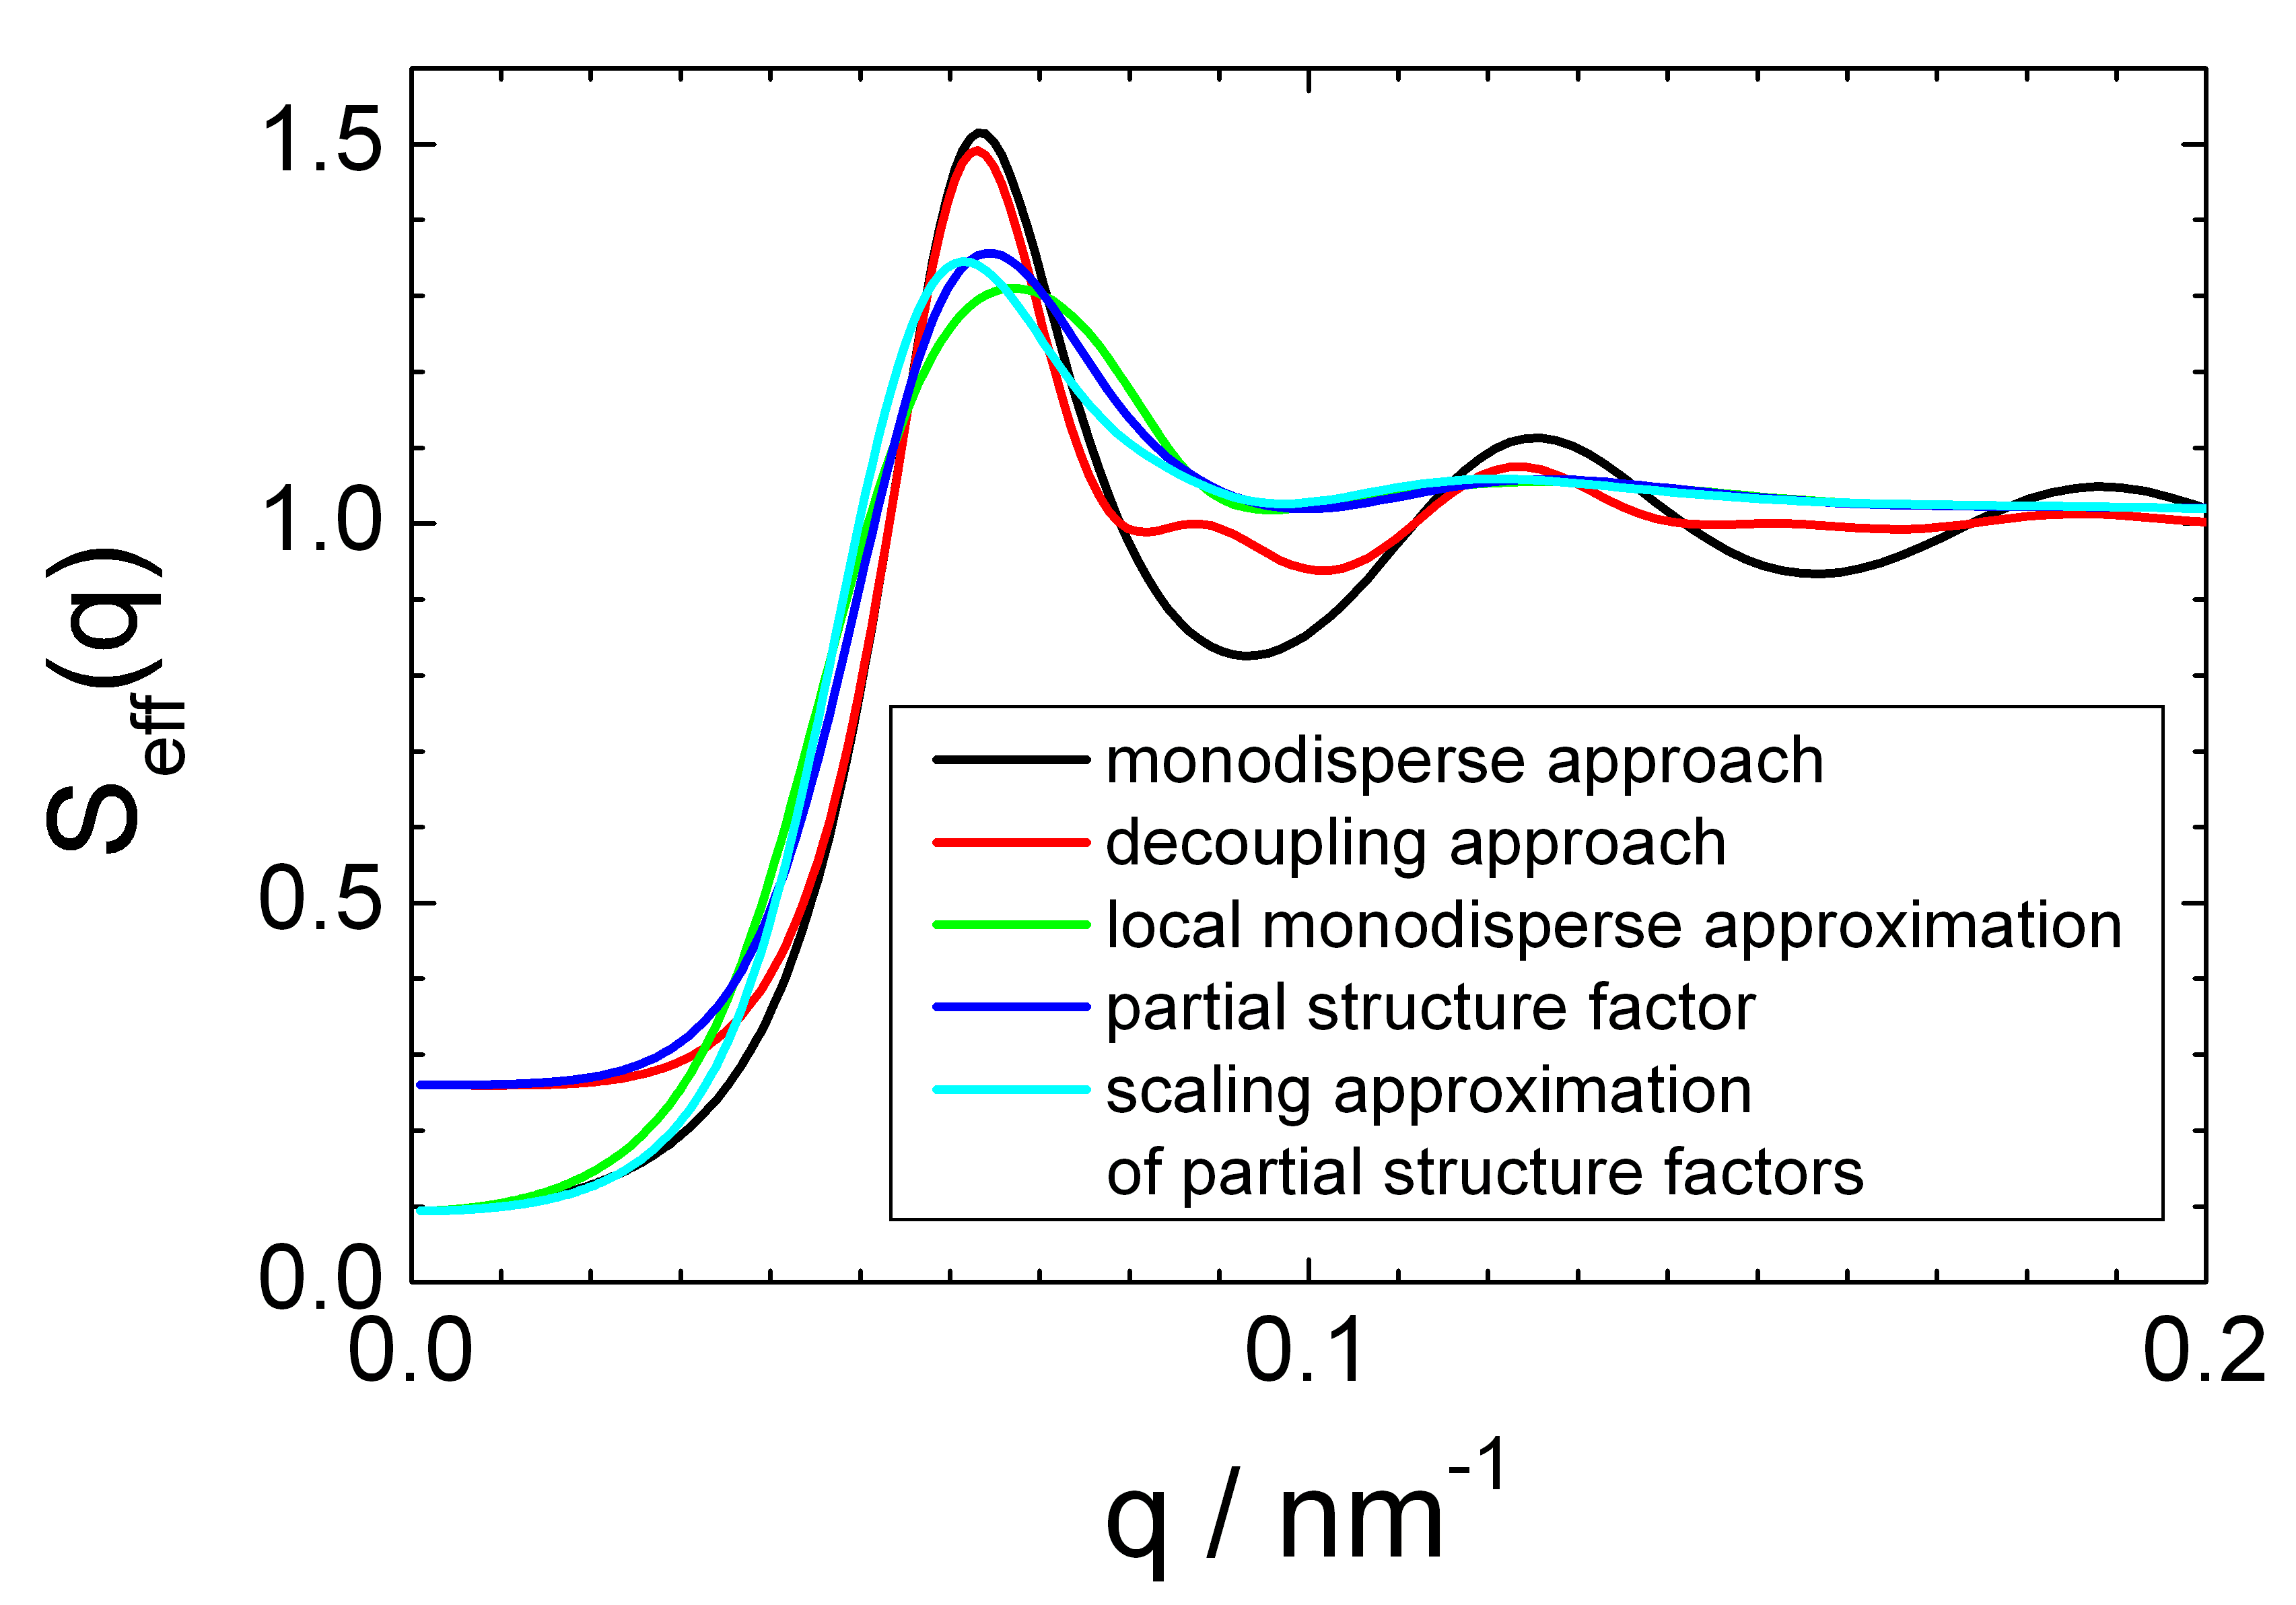
\includegraphics[width=0.65\textwidth]{../images/structure_factor/Seff.png}
\end{center}
\caption{Effective structure factor $S_\text{eff}(q)$ for Spheres with Hard Sphere interaction potential.
The fraction is assumed to be $\eta=0.3$. A LogNormal distribution with $\sigma=0.15$ and $R_0=50nm$
is assumed.}
\label{fig:Seff}
\end{figure}

\clearpage
\section{Hard \& Sticky Hard Sphere}
\subsection{Hard Sphere} \cite{Percus1958,Vrij1979}

\begin{equation}
U(r) =
 \begin{cases}
      \infty    & \text{for} \quad 0<r<\sigma \\
      0         & \text{for} \quad r>\sigma
   \end{cases}
\end{equation}

\begin{subequations}
\begin{align}
\alpha &= \frac{\left(1+2f_p\right)^2}{\left(1-f_p\right)^4} \\
\beta  &= -6 f_p \frac{\left(1 +f_p/2 \right)^2}{\left(1-f_p\right)^4} \\
\gamma &= \frac{f_p \alpha}{2}  \\
A &= 2 R_\text{HS} q
\end{align}

\begin{align}
G(f_p,A) =  & \, \alpha \, \frac{\sin A -A \cos A }{A^2} + \beta \, \frac{2 A \sin A +(2-A^2) \cos A -2}{A^3} + \nonumber \\
    & \, \gamma  \, \frac{-A^4 \cos A + 4\left[(3A^2-6)\cos A+(A^3-6A)\sin A+6\right]}{A^5}
\end{align}
\begin{align}
S_\text{HS}(q,R_\text{HS},f_p)  = & \cfrac{1}{1+24 f_p
\cfrac{G(f_p,A)}{A}}
\end{align}
\end{subequations}


\begin{figure}[htb]
\begin{center}
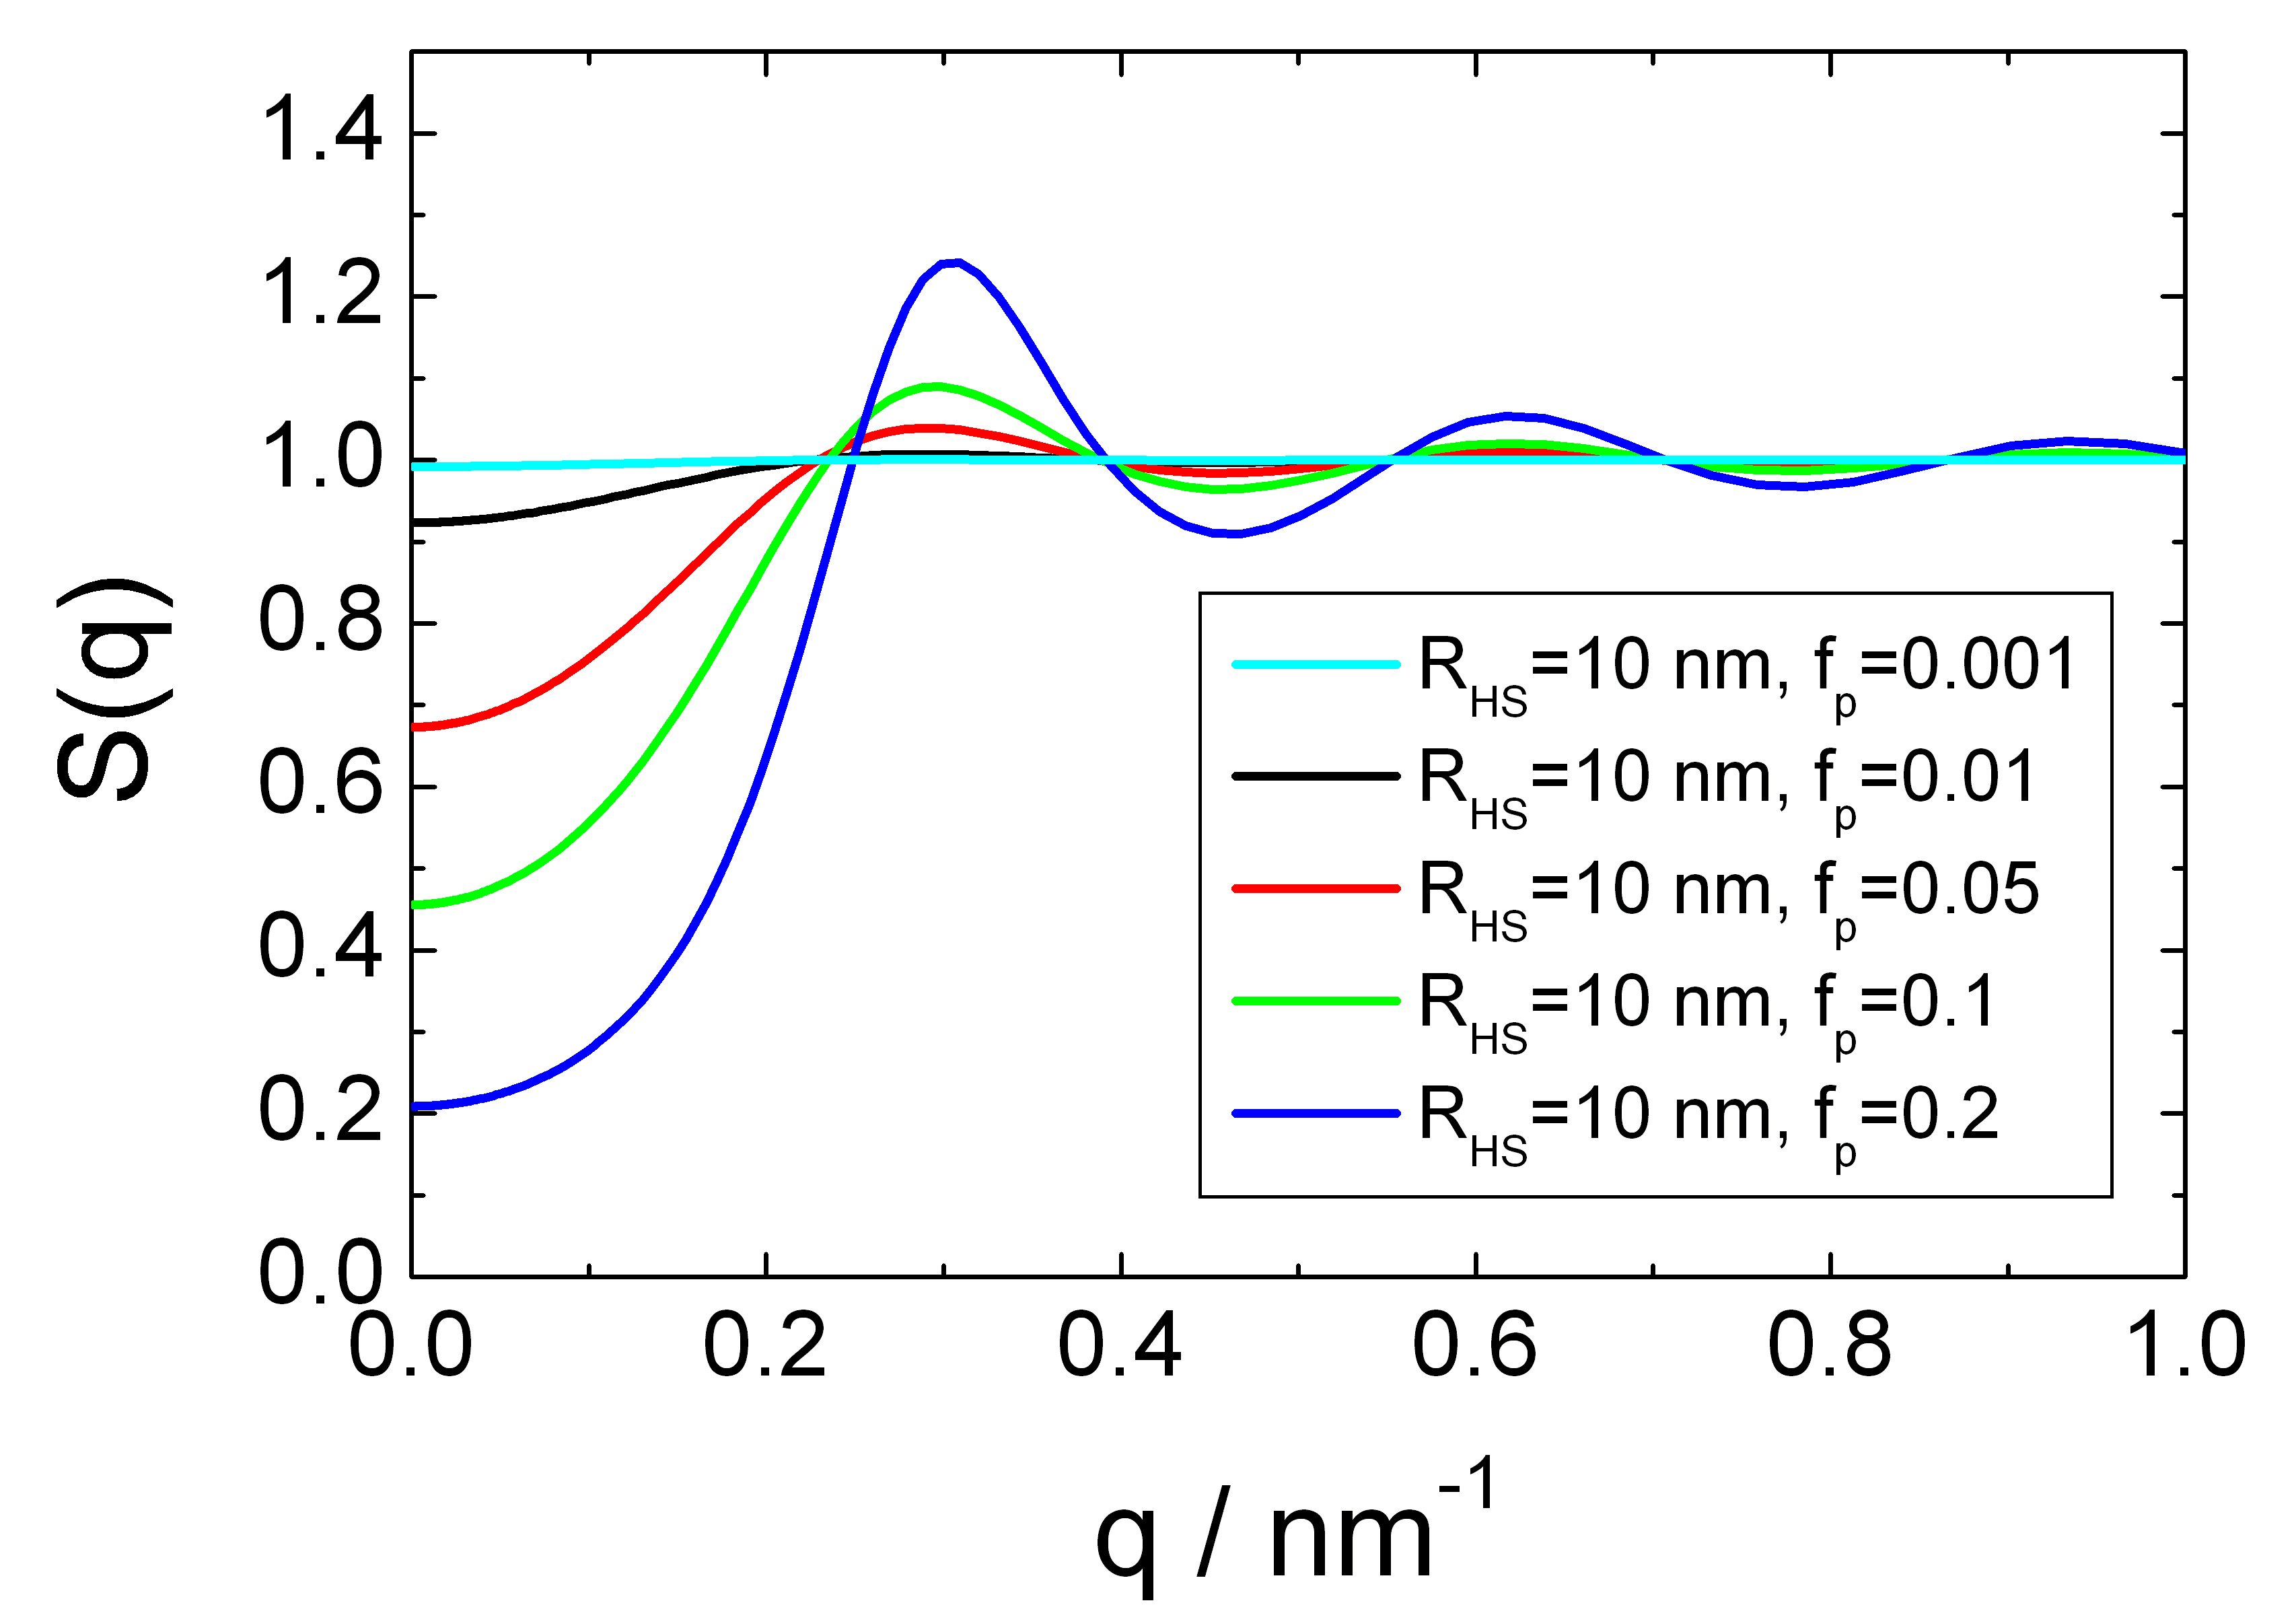
\includegraphics[width=0.768\textwidth]{../images/structure_factor/HardSphere/HardSphereSQ.png}
\end{center}
\caption{Structure factor $S(q)$ for a hard sphere interaction potential for the different volume fractions $f_p$.}
\label{fig:SQHardSphere}
\end{figure}


%%%%%%%%%%%%%%%%%%%%%%%%%%%%%%%%%%%%%%%%%%%%%%%%%%%%%%%%%%%%%%%%%%%%%%%%%%%%%%%%%%%%%%

\clearpage
\subsection{Sticky Hard Sphere} ~\\

In Baxter's model \cite{Baxter1968,Robertus1989,Kruif1989,Barboy1974,Menon1991,Menon1991a}
of adhesive hard spheres the pair interaction potential $U(r)$ is replaced by
\begin{equation}
\frac{U(r)}{k_BT} =
 \begin{cases}
      \infty    & \text{for} \quad 0<r<\sigma \\
      \ln\frac{12\tau\Delta}{\sigma+\Delta} & \text{for} \quad \sigma<r<\sigma+\Delta \\
      0         & \text{for} \quad r>\sigma+\Delta
   \end{cases}
\end{equation}
after which, when applied, the limit $\Delta \to 0$ is taken.
Thus, only a single parameter, the so-called stickiness parameter
$\tau$, characterizes the adhesive strength.
\begin{subequations}
\begin{align}
\kappa &= 2 q R_\text{HS} \\
\eta &= f_p \left(\frac{2R_\text{HS}+\Delta}{2R_\text{HS}}\right)^3\\
\epsilon &= \tau+\frac{\eta}{1-\eta} \\
\gamma &= f_p\frac{1+\eta/2}{3\left(1-\eta\right)^2} \\
\lambda &= \frac{6}{\eta} \left(\epsilon-\sqrt{\epsilon^2-\gamma}\right)\\
\mu &= \lambda \eta (1-\eta) \\
\beta &= -\frac{3\eta \left(2+\eta\right)^2-2\mu \left(1+7\eta+\eta^2\right)+\mu^2(2+\eta)}{2\left(1-\eta\right)^4}\\
\alpha &= \frac{\left(1+2\eta-\mu\right)^2}{\left(1-\eta\right)^4}\\[5mm]
C(q) = & 2\frac{\eta\lambda}{\kappa}\sin\kappa
        -2\frac{\eta^2\lambda^2}{\kappa^2}\left(1-\cos\kappa\right) -\\
   \Big\{ & \alpha\kappa^3(\sin\kappa-\kappa\cos\kappa)
           +\beta\kappa^2(2\kappa\sin\kappa-(\kappa^2-2)\cos\kappa-2)\nonumber\\
          & +\frac{\eta\alpha}{2}\left((4\kappa^3-24\kappa)\sin\kappa-(\kappa^4-12\kappa^2+24)\cos\kappa+24\right)
             \Big\} \;\times\;24\frac{\eta}{\kappa^6}\nonumber
\end{align}
\begin{align}
   S_\text{sHS}(q,R_\text{HS},f_p,\tau) & = \frac{1}{1-C(q)}
\end{align}
\end{subequations}



\begin{figure}[htb]
\begin{center}
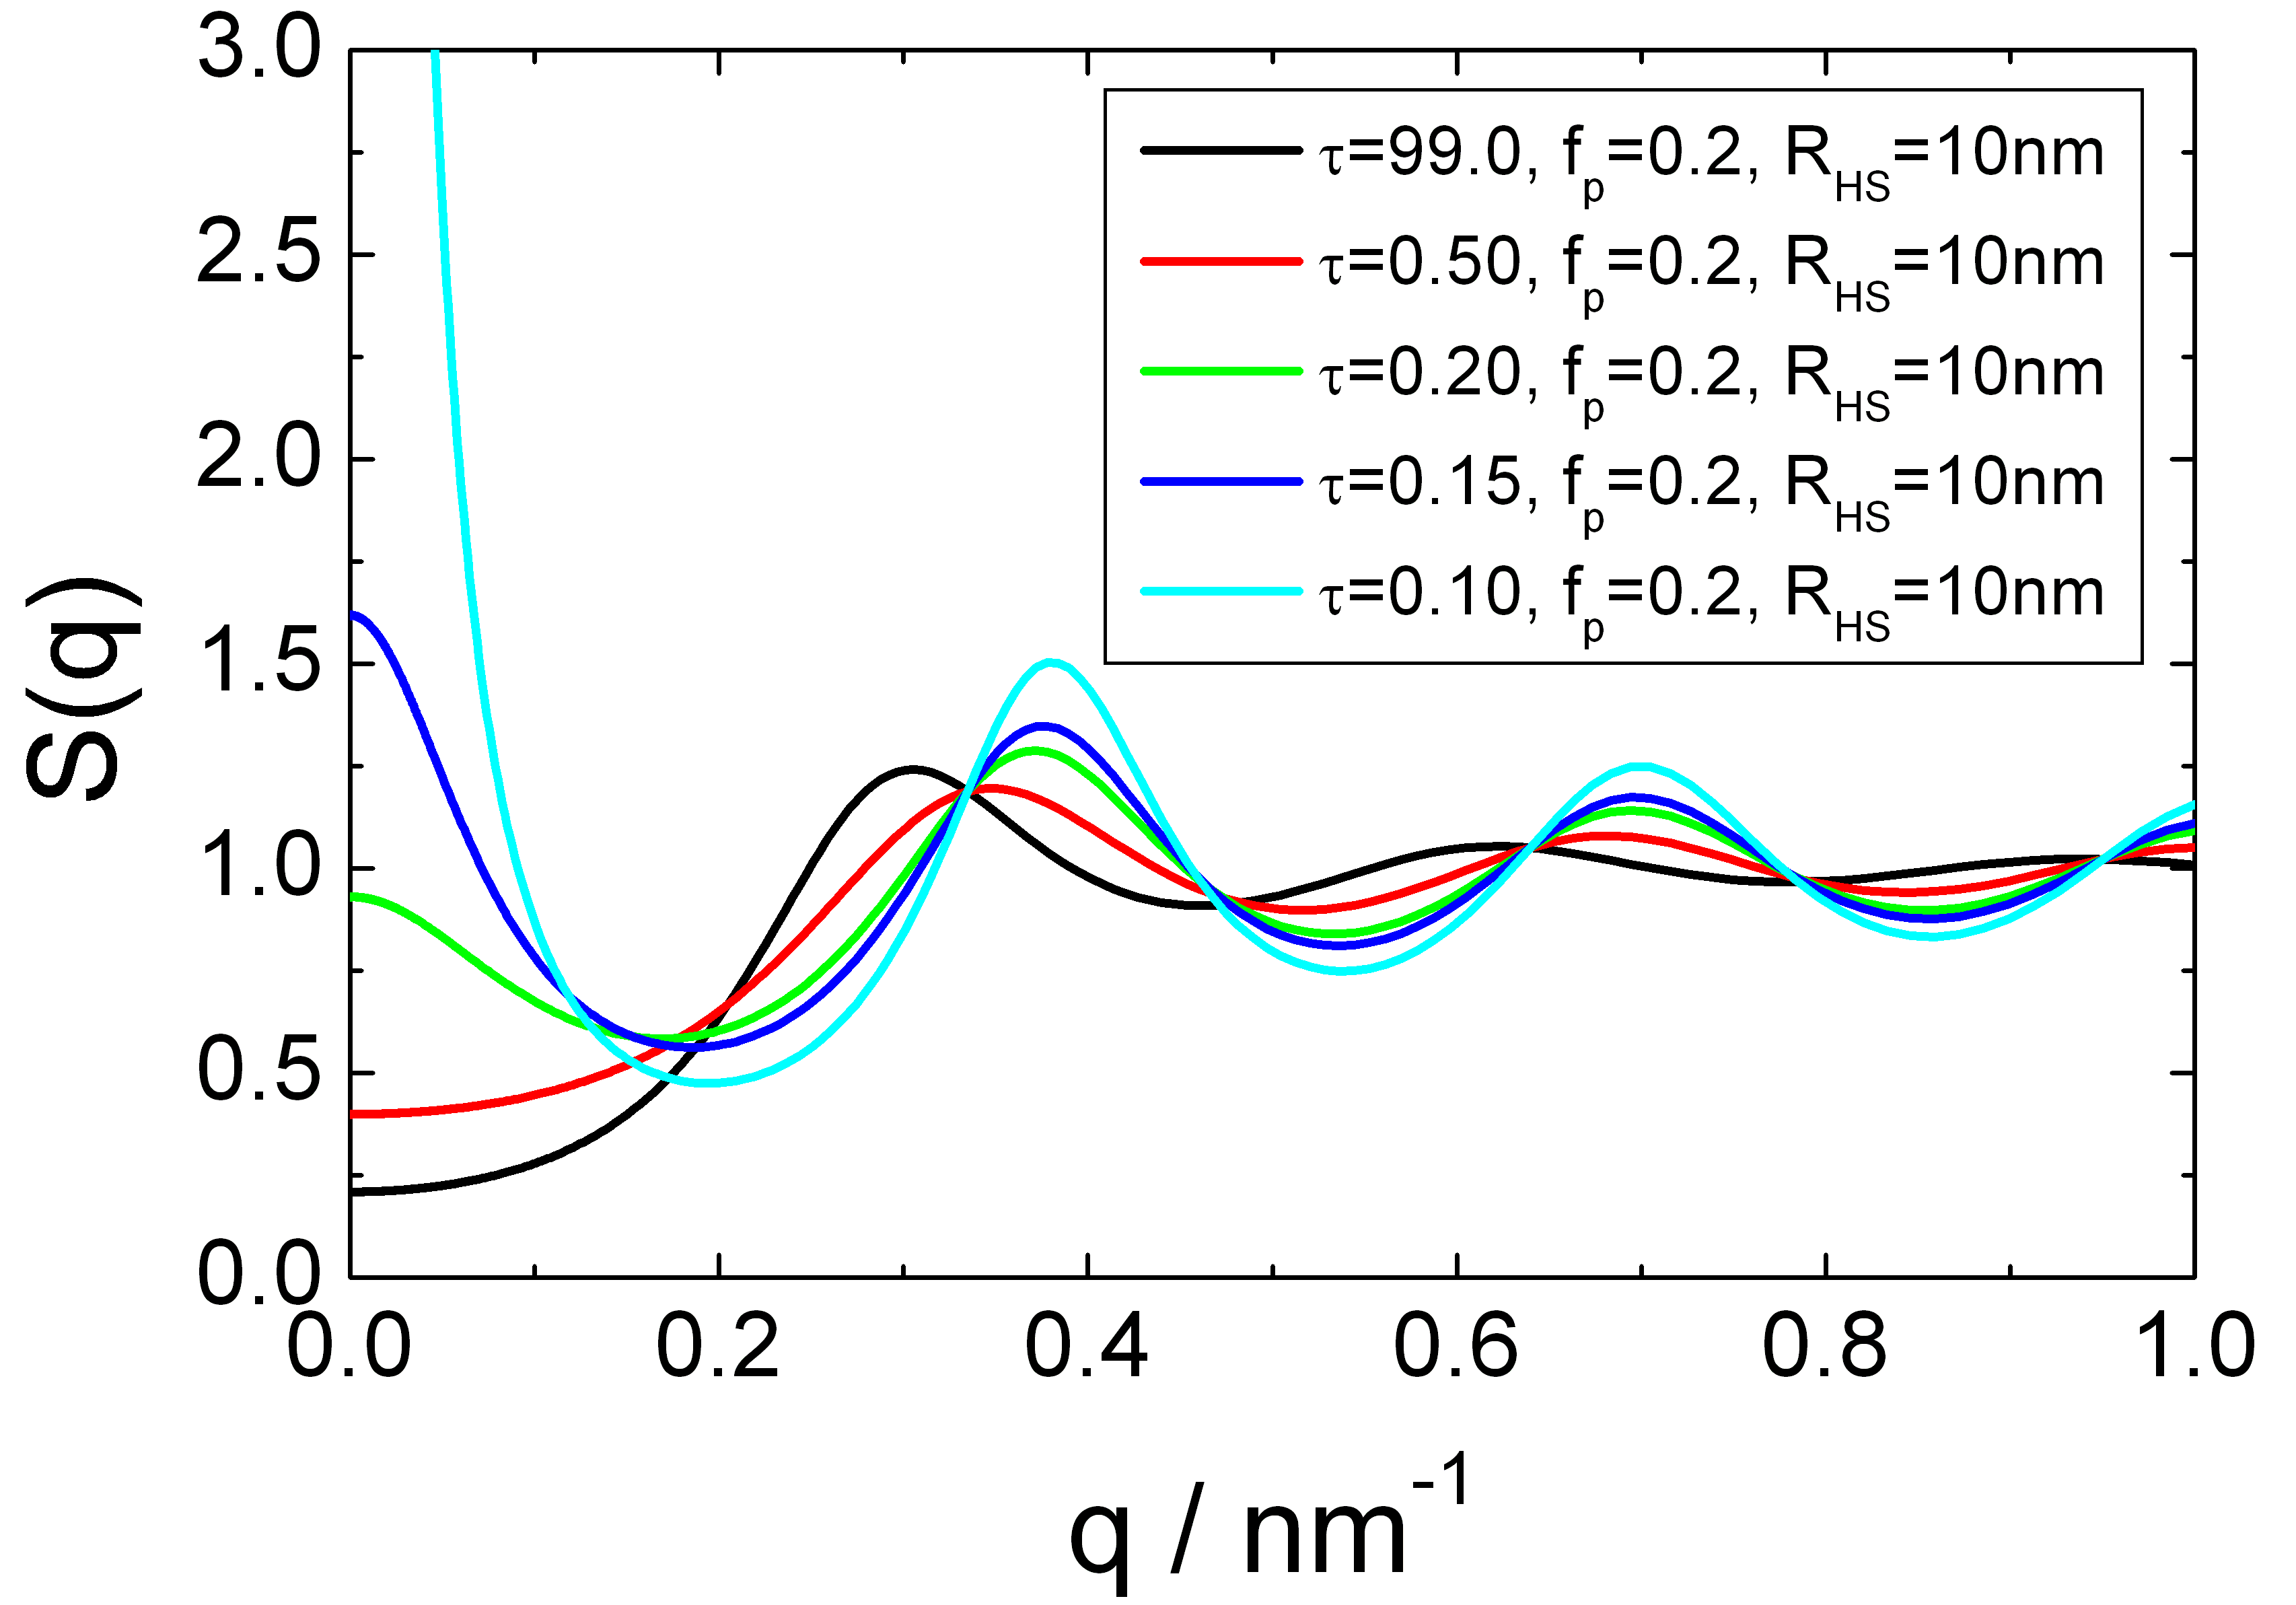
\includegraphics[width=0.768\textwidth]{../images/structure_factor/HardSphere/StickyHardSphere1.png}
\end{center}
\caption{Structure factor $S(q)$ for a sticky hard sphere interaction potential for the different
stickiness parameters $\tau$.}
\label{fig:SQStickyHardSphere1}
\end{figure}
%%%%%%%%%%%%%%%%%%%%%%%%%%%%%%%%%%%%%%%%%%%%%%%%%%%%%%%%%%%%%%%%%%%%%%%%%%

\clearpage
\subsection{Sticky Hard Sphere ($2^\text{nd}$ version)} \cite{Regnaut1989,Regnaut1990}~\\

In Baxter's model of adhesive hard spheres the pair interaction
potential $U(r)$ is replaced by
\begin{equation}
\frac{U(r)}{k_BT} =
 \begin{cases}
      \infty    & \text{for} \quad 0<r<\sigma-\Delta \\
      \ln\frac{12\tau\Delta}{\sigma+\Delta} & \text{for} \quad \sigma-\Delta<r<\sigma \\
      0         & \text{for} \quad r>\sigma
   \end{cases}
\end{equation}



\begin{align}
\sigma &= 2R_\text{HS}+\Delta \\
\kappa & = q \sigma \\
\phi   &= f_p \left(\frac{\sigma}{2R_\text{HS}}\right)^3 \\
\lambda_{\pm} & =6 \left(\frac{\tau}{\phi}+\frac{1}{1-\phi}\right)
                \pm \sqrt{
                    36 \left[
                        \frac{\tau}{\phi}+\frac{1}{1-\phi}
                      \right]^2
                   -\frac{12}{\phi}\frac{1+\frac{\phi}{2}}{\left(1-\phi\right)^{2}}
                } \\
   \lambda & =
       \begin{cases}
           \lambda_+ & \mbox{for }\lambda_+ < \abs{\lambda_-} \\
           \lambda_- & \mbox{otherwise}
       \end{cases}
\\[5mm]
\mu & = \lambda \phi (1-\phi) \\
A & = \frac12 \; \frac{1+2 \phi-\mu}{\left(1-\phi\right)^2} \\
B & = \frac{\sigma}{2} \frac{\mu-3\phi}{2 \left(1-\phi\right)^2 } \\
C & = -A\sigma^2-B\sigma+\lambda\sigma^2/12 \\
I_n(\kappa) &= \int_0^1 x^n \cos(\kappa x)\; dx \\
J_n(\kappa) &= \int_0^1 x^n \sin(\kappa x)\; dx \\
\alpha & = 1-12 f_p \left( C\sigma^{-2}I_0(\kappa) + B\sigma^{-1} I_1(\kappa) +AI_2(\kappa) \right)\\
\beta  &=    12 f_p \left( C\sigma^{-2}J_0(\kappa) + B\sigma^{-1} J_1(\kappa) +AJ_2(\kappa) \right) \\
S(Q) & = \frac{1}{\alpha^2+\beta^2}
\end{align}


\begin{figure}[htb]
\begin{center}
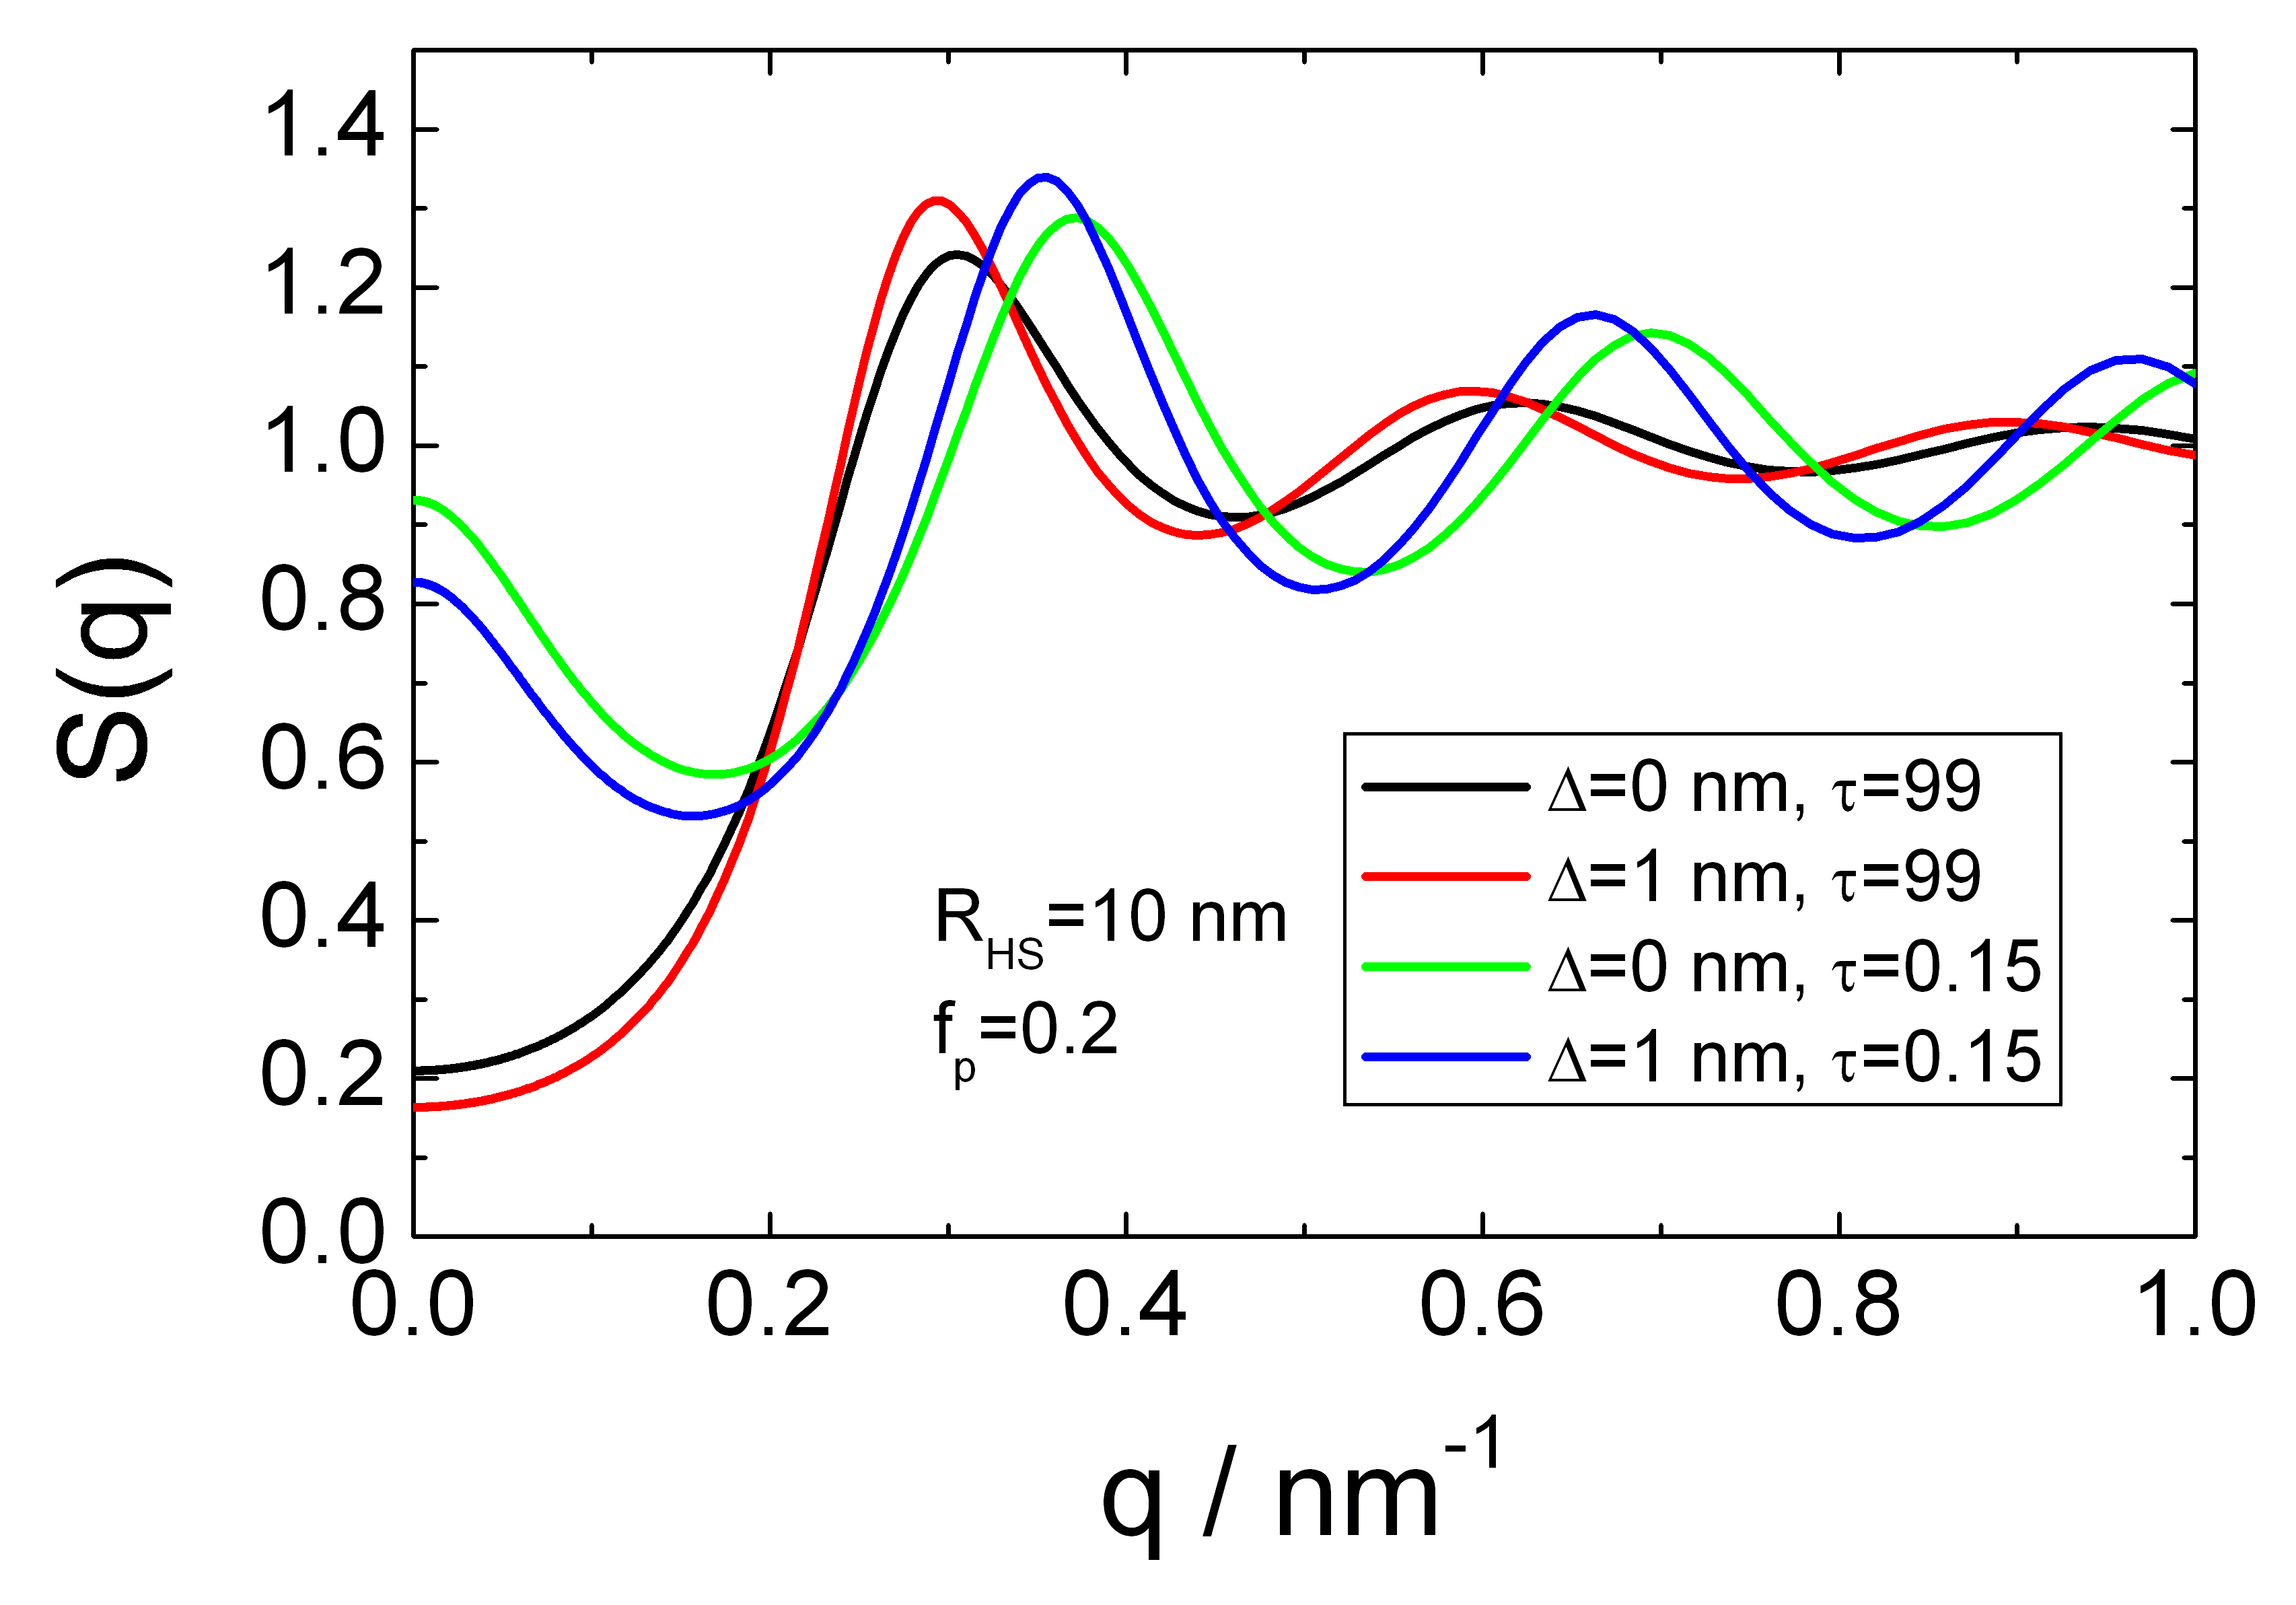
\includegraphics[width=0.768\textwidth]{../images/structure_factor/HardSphere/StickyHardSphere2.png}
\end{center}
\caption{Structure factor $S(q)$ for a sticky hard sphere interaction potential for the different
stickiness parameters $\tau$.}
\label{fig:SQStickyHardSphere2}
\end{figure}

%%%%%%%%%%%%%%%%%%%%%%%%%%%%%%%%%%%%%%%%%%%%%%%%%%%%%%%%%%%%%%%%%%%%%%%%%%%%%%%%%%%%%

\clearpage
\subsection{Square Well Potential}  \cite{Sharma1977}~\\

The Square well potential can be written as
\begin{equation}
U(r) =
 \begin{cases}
      \infty    & \text{for} \quad 0<r<\sigma \\
      -\epsilon & \text{for} \quad \sigma<r<\lambda\sigma \\
      0         & \text{for} \quad r>\lambda\sigma
   \end{cases}
\end{equation}
where $\lambda$ and $\epsilon$ correspond to the breadth and the
depth of the square well potential. The structure factor $S(Q)$ is
then given by the following relations:
\begin{subequations}
\begin{align}
S(Q)  = & \frac{1}{1-C(Q)} \\
C(Q)  = & - \frac{24\eta}{(Q\sigma)^6} \Big\{ \alpha(Q\sigma)^3
\left[\sin(Q\sigma)-Q\sigma\cos(Q\sigma)\right] \\
        & +\beta(Q\sigma)^2\left[2Q\sigma\sin(Q\sigma)-(Q^2\sigma^2-2)\cos(Q\sigma)-2\right]\nonumber\\
        & +\gamma \left[(4Q^3\sigma^3-24Q\sigma)\sin(Q\sigma)-(Q^4\sigma^4-12Q^2\sigma^2+24)\cos(Q\sigma)+24\right] \nonumber\\
        & -\frac{\epsilon}{k_BT} (Q\sigma)^3\left[\sin(\lambda Q\sigma)-\lambda Q\sigma\cos(\lambda Q\sigma)+Q\sigma\cos(Q\sigma)-\sin(Q\sigma)\right]\Big\} \nonumber
\end{align}
where $\alpha$, $\beta$ and $\gamma$ are given by
\begin{align}
\alpha & = \frac{(1+2\eta)^2+\eta^3(\eta-4)}{(1-\eta)^4} \\
\beta  & = -\frac{1}{3}\eta\frac{18+20\eta-12\eta^2+\eta^4}{(1-\eta)^4} \\
\gamma & =
\frac{1}{2}\eta\frac{(1+2\eta)^2+\eta^3(\eta-4)}{(1-\eta)^4}
\end{align}
\end{subequations}
~\\
NOTE:\\
Values for the depth of $\epsilon>1.5k_BT$ and for the volume
fraction of $\eta> 0.08$ may give unphysical results when
compared to Monte Carlo simulations according to \cite{Sharma1977}.

\begin{figure}[htb]
\begin{center}
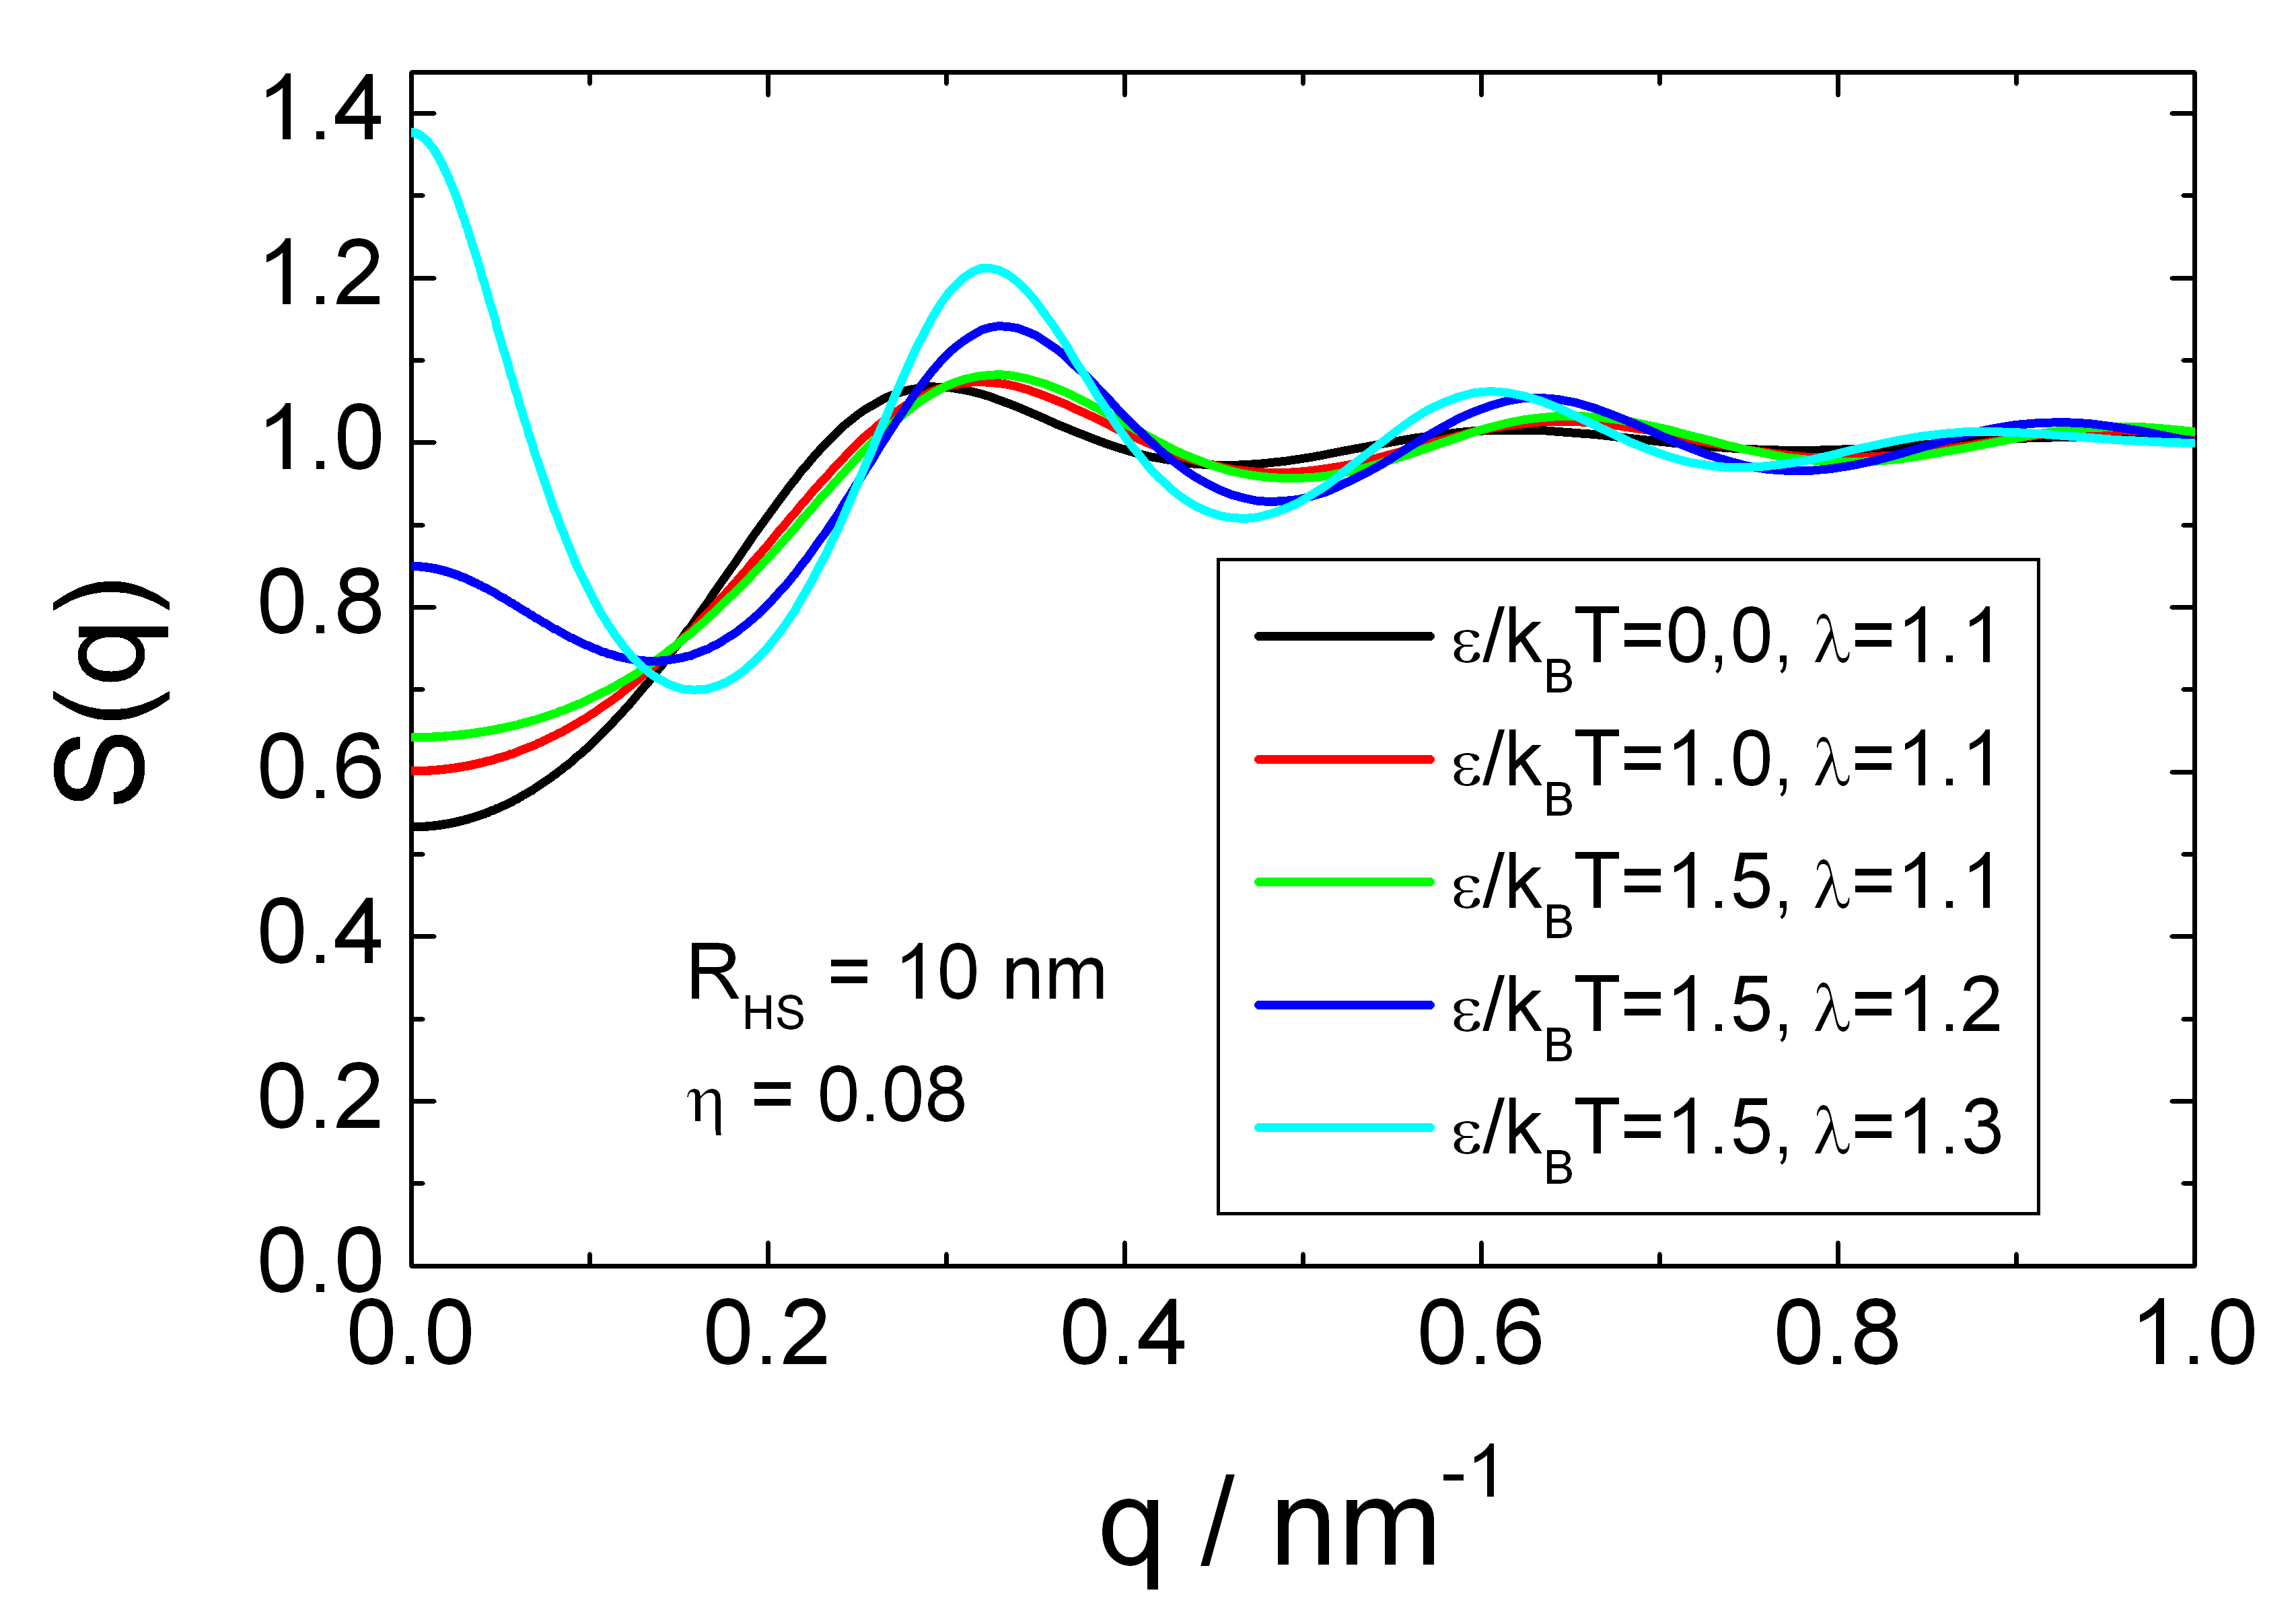
\includegraphics[width=0.768\textwidth]{../images/structure_factor/HardSphere/SquareWellSQ.png}
\end{center}
\caption{Structure factor $S(q)$ for a square well interaction potential.}
\label{fig:SquareWell1}
\end{figure}

%%%%%%%%%%%%%%%%%%%%%%%%%%%%%%%%%%%%%%%%%%%%%%%%%%%%%%%%%%%%%%%%%%%%%%%%%%%%%%%%%%

\clearpage
\subsection{Square Well Potential 2} ~\\

The Square well potential can be written as
\begin{equation}
U(r) =
 \begin{cases}
      \infty    & \text{for} \quad 0<r<\sigma \\
      -\epsilon & \text{for} \quad \sigma<r<\sigma+\Delta \\
      0         & \text{for} \quad r>\sigma+\Delta
   \end{cases}
\end{equation}
where $\Delta$ and $\epsilon$ correspond to the width and the
depth of the square well potential. The structure factor $S(Q)$ is
then given by the following relations:
\begin{equation}
S(Q)  = 1
-4\pi\rho\sigma^3\frac{\sin(Q\sigma)-Q\sigma\cos(Q\sigma)}{Q^3\sigma^3}
          +4\pi\rho\sigma^2\left[e^{\frac{\epsilon}{k_BT}}-1\right]\frac{\sin(Q\sigma)}{Q\sigma}
          \Delta
\end{equation}
where $\sigma$ is the particle diameter ($R_{HS} = \sigma/2$: hard
sphere radius is requested by software as input parameter),
$\Delta$ the width of the square well potential, $\epsilon$ (input
value in software is $\epsilon/k_B$, i.e. in Kelvin), $T$ (in
Kelvin) the sample temperature, the depth and $\rho$ the colloid
concentration, which is related to the colloid volume fraction
$\eta$ by $\eta=\pi\rho\sigma^3/6$.




%%%%%%%%%%%%%%%%%%%%%%%%%%%%%%%%%%%%%%%%%%%%%%%%%%%%%%%%%%%%%%%%%%%%%%%%%%%%
\clearpage
\section{Other Structure Factors}

\subsection{Hayter-Penfold RMSA }

This is the structure factor for a system of charged, spheroidal objects in a dielectric
medium \cite{Hayter1981,Hansen1982}. When
combined with an appropriate form factor (such as sphere, core+shell, ellipsoid etc.),
this allows for inclusion of the interparticle interference effects due to screened
coulomb repulsion between charged particles.
The salt concentration, is used to compute the ionic strength of the solution which
in turn is used to compute the Debye screening length. At present there is no provision
for entering the ionic strength directly nor for use of any multivalent salts. The
counterions are also assumed to be monovalent.



\hspace{1pt}\\
\underline{Input Parameters for model \texttt{Hayter Penfold RMSA}:}\\
\begin{description}
\item[\texttt{RHS}] hard sphere radius $R_{HS}$ of particles in [nm].
\item[\texttt{Z}] charge of particle in units of the charge of an electron $e=-1.602 176 620 8 \times 10^{-19} \mathrm{C}$
\item[\texttt{eta}] volume fraction $\eta$ of particles
\item[\texttt{T}] sample temperature $T$ in Kelvin
\item[\texttt{salt}] monovalent salt concentration in [M]
\item[\texttt{eps\_r}] dielectric constant $\epsilon_r$ of solvent (vacuum:1, water at $25^\circ$: 78.2, water at $20^\circ$: 80.4, ethanol at $20^\circ$: 25.16, toluene at $23^\circ$: 2.38)
\end{description}

%\vspace{5mm}
%\noindent REFERENCE\\
%1. JP Hansen and JB Hayter "A rescaled MSA structure factor for dilute charged
%colloidal dispersions" Molecular Physics 46, 651-656 (1982).\\
%2. JB Hayter and J Penfold "An analytic structure factor for macroion solutions"
%Molecular Physics 42, 109-118 (1981)

%%%%%%%%%%%%%%%%%%%%%%%%%%%%%%%%%%%%%%%%%%%%%%%%%%%%%%%%%%%%%%%%%%%%%%%%%%%%

\clearpage
\subsection{MacroIon}

\begin{subequations}
\begin{align}
ETA &= \text{volume fraction} \\
AK &= \kappa \sigma = \text{inv. screening length times diameter} \\
\kappa &=\sqrt{ e^2/(\epsilon \epsilon_0 k_B T)*(\rho_c+2 \rho_s) }\\
\rho_c &= \text{density of counterions} = \rho_\text{colloids} Z \\
\rho_s &= \text{density of salt cations or anions} \\
GEK &=\text{charge}^2/( \pi k_B T \epsilon \epsilon_0 \sigma (2+AK)^2)\\
\text{charge} &= \text{Ladung eines Kolloids} = e Z\\
S=ETA^{1./3} &= \text{scaling factor for rescaled MSA (RMSA)}\\
GAMK&=2*S*GEK*\exp(AK-AK/S).
\end{align}
\end{subequations}

%%%%%%%%%%%%%%%%%%%%%%%%%%%%%%%%%%%%%%%%%%%%%%%%%%%%%%%%%%%%%%%%%%%%%%%%%%%%

\clearpage
\subsection{Critical Scattering}

\BE S_\text{crit}(Q)=1+\frac{\kappa}{1+\zeta^2Q^2} \EE $\zeta$:
correlation length, $\kappa$: scaling factor


%%%%%%%%%%%%%%%%%%%%%%%%%%%%%%%%%%%%%%%%%%%%%%%%%%%%%%%%%%%%%%%%%%%%%%%%%%%%

%\subsection{Correlation Hole}
%\BE S_\text{corr. hole}(Q,h,\eta)=1+\eta \Phi(Qh) \EE $\Phi(x) =
%3\frac{\sin(x)-x\cos(x)}{x^3}$ $\eta$: volume fraction, $h$: hole
%radius

%%%%%%%%%%%%%%%%%%%%%%%%%%%%%%%%%%%%%%%%%%%%%%%%%%%%%%%%%%%%%%%%%%%%%%%%%%%%

%\subsection{Random Distribution Model}

%(eq.\ 75 in \cite{Guinier1963} )
%\BE S_\text{RDM}(Q) =
%\frac{1}{1+8 f_P\epsilon\Phi(x)} \EE
%$x = 2QR_{ca}$ \\
%$\epsilon$: which designates a constant approximately equal to unity\\
%$f_P =v_0/v_1 $ \\
%$v_{0} = \frac{4}{3}\pi R_{ca}^3$: particle volume\\
%$v_1  = \frac{V_0}{N_0}$:  average volume offered each particle \\
%$\Phi(x) = 3\frac{\sin(x)-x\cos(x)}{x^3}$\\
%~\\


%\subsection{Local Order Model}
%\cite{Mauritz2004}
%\BE S_\text{LOM}(Q) = 1+4\frac{\sin(QD)}{QD}-z\Phi(x); \EE
%$x = \alpha Q D$\\
%$\Phi(x) = 3\frac{\sin(x)-x\cos(x)}{x^3}$

%%%%%%%%%%%%%%%%%%%%%%%%%%%%%%%%%%%%%%%%%%%%%%%%%%%%%%%%%%%%%%%%%%%%%%%%%%%%

\subsection{Cylinder(PRISM)}

\BE S_\text{Cyl,PRISM} = \frac{1}{1+\nu C_q P_{15}} \EE
$x = 2QR$ \\[3mm]
$x_{P15} = Q(L-2R)$ \\[3mm]
$\displaystyle P_{15} = 2\frac{\text{Si}(x_{P15})}{x_{P15}} - 4\frac{\sin^2(x_{P15}/2)}{x_{P15}^2}$ \\[3mm]
$\displaystyle C_q = 3\frac{\sin(x)-x\cos(x)}{x^3}$ \\

%%%%%%%%%%%%%%%%%%%%%%%%%%%%%%%%%%%%%%%%%%%%%%%%%%%%%%%%%%%%%%%%%%%%%%%%%%%%

\clearpage
\subsection{Voigt Peak} ~\\

In spectroscopy, the Voigt profile is a spectral line profile
named after Woldemar Voigt and found in all branches of
spectroscopy in which a spectral line is broadened by two types of
mechanisms, one of which alone would produce a Doppler profile,
and the other of which would produce a Lorentzian profile. All
normalized line profiles can be considered to be probability
distributions. The Doppler profile is essentially a normal
distribution and a Lorentzian profile is essentially a Cauchy
distribution. Without loss of generality, we can consider only
centered profiles which peak at zero. The Voigt profile is then
the convolution of a Lorentzian profile and a Doppler profile:
\begin{subequations}
\begin{align}
V(x\vert\sigma,\gamma)& = \int_\infty^\infty D(x'\vert\sigma) \,
                                            L(x-x'\vert\gamma)\, dx'
\end{align}
where $x$ is frequency from line center, $D(x\vert\sigma)$ is the
centered Doppler profile:
\begin{align}
D(x\vert\sigma) & = \frac{e^{-x^2/2\sigma^2}}{\sigma\sqrt{2\pi}}
\end{align}
and $L(x\vert\gamma)$ is the centered Lorentzian profile:
\begin{align}
L(x\vert\gamma) & = \frac{\gamma}{\pi(x^2+\gamma^2)} .
\end{align}
The defining integral can be evaluated as:
\begin{align}
V(x) & = \frac{\Re[w(z)]}{\sigma\sqrt{2\pi}}
\end{align}
where $\Re[w(z)]$ is the real part of the complex error function
of $z$ and
\begin{align}
z = \frac{x+i\gamma}{\sigma\sqrt{2}}
\end{align}
\begin{align}
S_{\text{Voigt}}(Q,Q_m,A,\sigma,\gamma,c_0) = A \,\,
V(Q-Q_m\vert\sigma,\gamma)+c_0
\end{align}
\end{subequations}

